\section{}
\[
H(s)=\frac{100\,s}{s+1}\,.
\]
\subsection{Bode-Diagramm}
\begin{center}
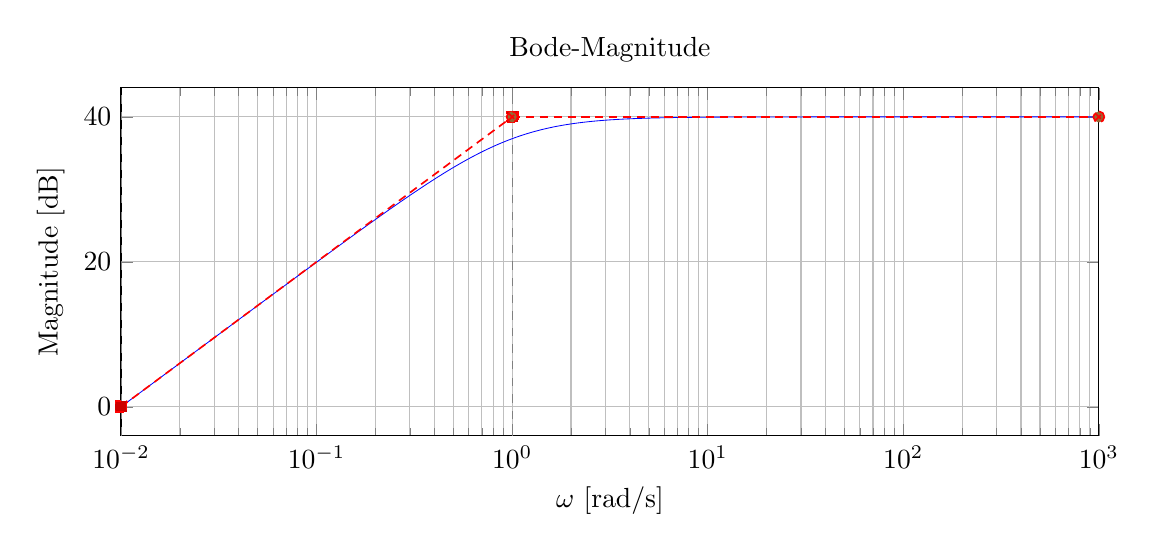
\begin{tikzpicture}
\begin{semilogxaxis}[
  width=14cm,height=6cm,
  xmin=1e-2,xmax=1e3,
  xlabel={$\omega$ [rad/s]},
  ylabel={Magnitude [dB]},
  grid=both,
  title={Bode-Magnitude}
]
\addplot[
  domain=1e-2:1e3,
  samples=600,
  mark=none,
  line width=0.3pt,
  blue
] {40 + 20*ln(x)/ln(10) - 20*ln(sqrt(1 + x^2))/ln(10)};
\addplot+[domain=1e-2:1,samples=2,dashed,dash pattern=on 3pt off 2pt,line width=0.6pt,red] {40 + 20*ln(x)/ln(10)};
\addplot+[domain=1:1e3,samples=2,dashed,dash pattern=on 3pt off 2pt,line width=0.6pt,red] {40};
\draw[gray,dashed] (rel axis cs:0,0) -- (rel axis cs:0,1);
\draw[gray,dashed] (axis cs:1,\pgfkeysvalueof{/pgfplots/ymin}) -- (axis cs:1,\pgfkeysvalueof{/pgfplots/ymax});
\node[gray,anchor=south east] at (axis cs:1,\pgfkeysvalueof{/pgfplots/ymax}) {\scriptsize Pol $\omega_p=1$};
\end{semilogxaxis}
\end{tikzpicture}
\vspace{6mm}
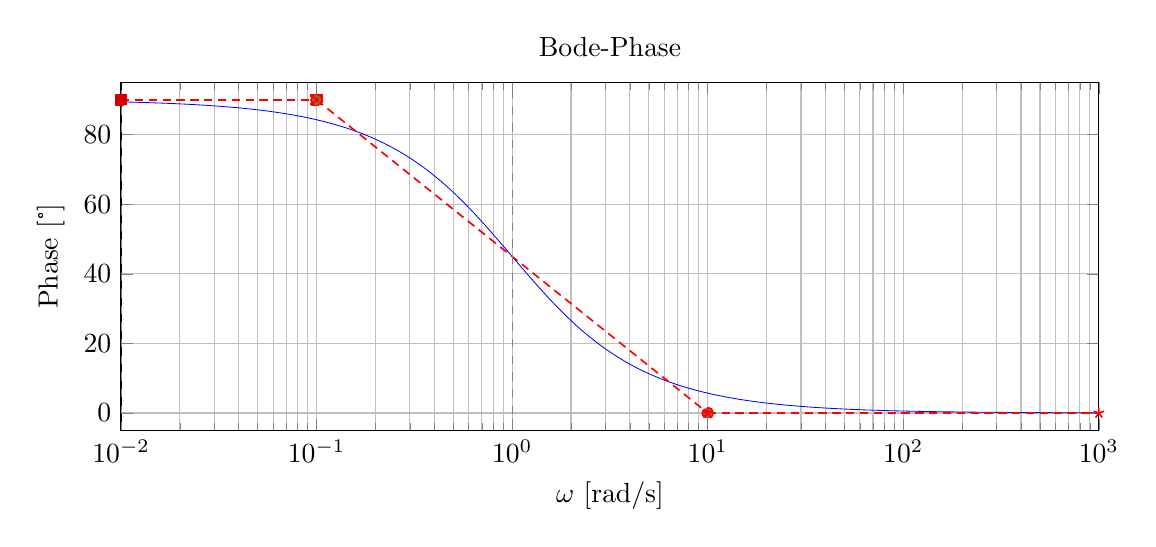
\begin{tikzpicture}
\begin{semilogxaxis}[
  width=14cm,height=6cm,
  xmin=1e-2,xmax=1e3,
  ymin=-5,ymax=95,
  xlabel={$\omega$ [rad/s]},
  ylabel={Phase [°]},
  grid=both,
  title={Bode-Phase}
]
\addplot[
  domain=1e-2:1e3,
  samples=600,
  mark=none,
  line width=0.3pt,
  blue
] {90 - atan(x)};
\addplot+[domain=1e-2:1e-1,samples=2,dashed,dash pattern=on 3pt off 2pt,line width=0.6pt,red] {90};
\addplot+[domain=1e-1:1e1,samples=2,dashed,dash pattern=on 3pt off 2pt,line width=0.6pt,red] {45 - 45*ln(x)/ln(10)};
\addplot+[domain=1e1:1e3,samples=2,dashed,dash pattern=on 3pt off 2pt,line width=0.6pt,red] {0};
\draw[gray,dashed] (rel axis cs:0,0) -- (rel axis cs:0,1);
\draw[gray,dashed] (axis cs:1,\pgfkeysvalueof{/pgfplots/ymin}) -- (axis cs:1,\pgfkeysvalueof{/pgfplots/ymax});
\node[gray,anchor=south east] at (axis cs:1,\pgfkeysvalueof{/pgfplots/ymax}) {\scriptsize Pol $\omega_p=1$};
\end{semilogxaxis}
\end{tikzpicture}
\end{center}
\newpage
\subsection{Erklärung}
\vspace{5mm}
\begin{description}[leftmargin=1.2em,labelsep=.6em,font=\bfseries]
\item[Schritt 1] DC-Faktor $100$: Betrag global um $+40\,\mathrm{dB}$ verschoben; die konstante (reell-positive) Verstärkung ändert die Steigung nicht und fügt keine zusätzliche Phase hinzu. Referenzniveau der Geradennäherung damit bei $40\,\mathrm{dB}$.
\item[Schritt 2] Nullstelle im Ursprung: Startsteigung $+20\,\mathrm{dB/dec}$ für $\omega\ll1$, da $|H(\j\omega)|\sim100\,\omega$; Startphase $\approx+90^\circ$ (ideale Integrationsumkehr). In der Magnituden-Näherung ergibt sich links der Ecke die Gerade $40+20\log_{10}\omega$.
\item[Schritt 3] Pol bei $\omega_p=1\,\mathrm{rad/s}$: ab $\omega=1$ Steigungswechsel um $-20\,\mathrm{dB/dec}$; resultierend flacht die Magnitude auf $0\,\mathrm{dB/dec}$ ab und nähert sich für $\omega\gg1$ dem konstanten Niveau $\approx40\,\mathrm{dB}$. Exakter Eckpunkt: $40-10\log_{10}2\approx36.99\,\mathrm{dB}$. Die Phase fällt über die Übergangsdekade $\omega_l=0.1$ bis $\omega_h=10\,\mathrm{rad/s}$ von $\approx+90^\circ$ gegen $0^\circ$ (Geradennäherung: $45^\circ-45^\circ\log_{10}\omega$ in $[0.1,10]$).
\end{description}

\vspace{0.5cm}
\medskip
\noindent\textbf{Stückweise Näherung}
\[
|H(\j\omega)|_{\mathrm{dB}}\approx
\begin{cases}
40+20\log_{10}\omega,& \omega\ll1,\\[4pt]
40-10\log_{10}2,& \omega=1,\\[4pt]
40,& \omega\gg1,
\end{cases}
\qquad
\]
\newpage